\begin{scanpage}{0183}{165}
\begin{minipage}[t]{.44\linewidth}\vspace{0pt}\centering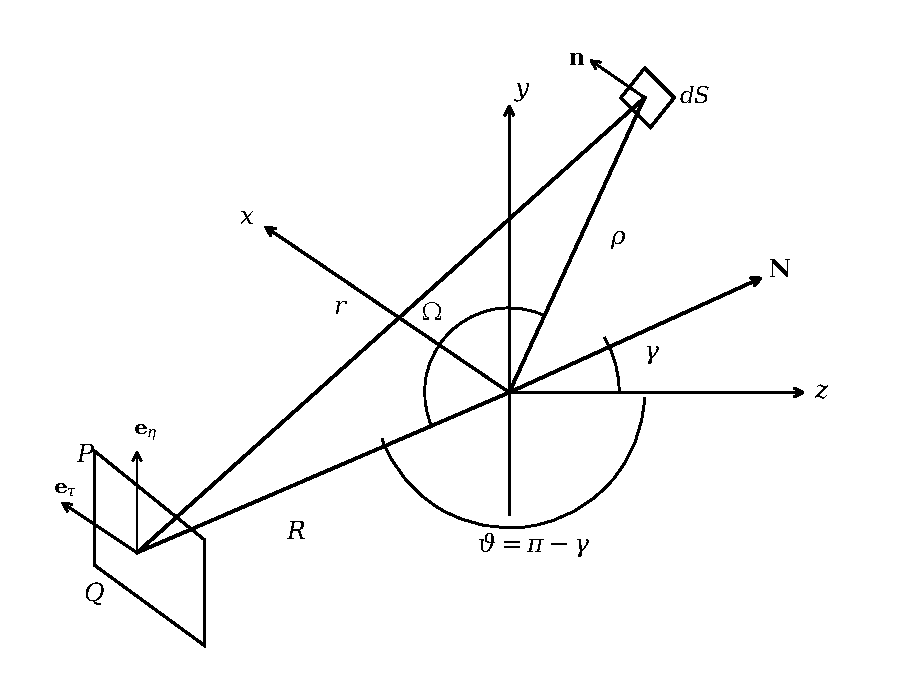
\includegraphics[width=.95\linewidth]{images/recreated/c-0183-fig69.pdf}\par\raggedright
Figure 69. The problem of electromagnetic wave diffraction by an arbitrary metal body.\par
dS -- is a surface element of the body.\par
N -- the normal to the incident wave front,\par
Q -- the source,\par
P -- the polarizer converting linearly polarized radiation to a wave with circular polarization.
\begin{center}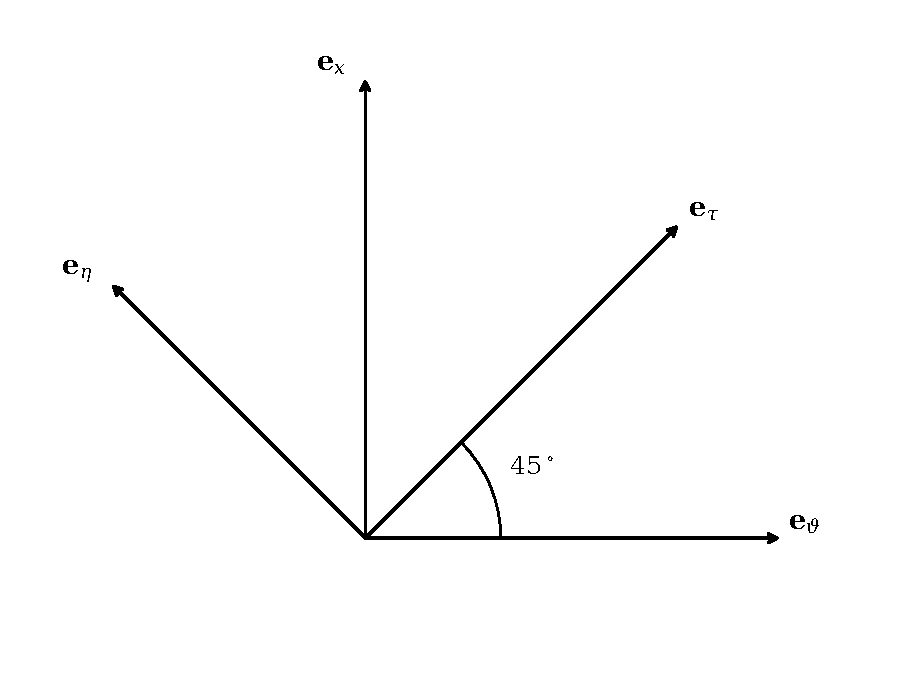
\includegraphics[width=.65\linewidth]{images/recreated/c-0183-fig70.pdf}\par Figure 70.\end{center}
\end{minipage}\hfill
\begin{minipage}[t]{.53\linewidth}\vspace{0pt}
field (26.03) is an elliptically polarized wave. In the direction toward the source ($\vartheta=\pi-\gamma$, $\varphi=-\pi/2$), this wave passes through the polarizer and creates behind it the field
\[
\left.\begin{aligned}E_x=-H_\vartheta&=\frac{iaE_{0x}}2\Sigma_+\frac{e^{ikR}}R e^{i\pi/2},\\
E_\vartheta=H_x&=\frac{iaE_{0x}}2\Sigma_-\frac{e^{ikR}}R.
\end{aligned}\right\}\tag{26.04}
\]
where
\[
\Sigma_\pm=\frac12(\Sigma\pm\overline\Sigma).\tag{26.05}
\]
If the source radiates a wave of another polarization ($\mathbf H_0\perp yoz$), then the wave reflected by the body and passing through the polarizer is described at the point Q by similar relationships
\[
\left.\begin{aligned}H_x=E_\vartheta&=\frac{iaH_{0x}}2\Sigma_+\frac{e^{ikR}}R e^{i\pi/2},\\
H_\vartheta=-E_x&=\frac{iaH_{0x}}2\Sigma_-\frac{e^{ikR}}R.
\end{aligned}\right\}\tag{26.06}
\]
\end{minipage}
\par Now let us investigate in the physical optics approach the diffraction of a plane linearly polarized wave by the same body. According to definition (3.01), the uniform part of the current excited on the body's surface by a plane wave with E-polarization of the incident wave ($\mathbf E_0\perp yoz$) equals
\end{scanpage}
